\documentclass[10pt,aspectratio=169]{beamer}

% All the boilerplate is in raslides.sty
% Note that this also pulls in a custom vogtwidebar.sty
\usepackage{raslides}

\author{Ji\v{r}\'i Lebl}

\institute[OSU]{%
Departemento pri Matematiko de Oklahoma {\^S}tata Universitato}

\title{BA: 1.2}

\date{}

\begin{document}

\begin{frame}
\titlepage
\end{frame}

\begin{frame}
We will simply assume that real numbers exist, that is, we won't prove:

\begin{theorem}
There exists a unique
ordered field $\R$ with the least-upper-bound property
such that $\Q \subset \R$.
\end{theorem}

\pause

We'll simply assume
simple properties that follow from the definition.

E.g.:

\medskip
\pause

$1 > 0$, $2 > 0$, ..., $n > 0$ for all $n \in \N \subset \R$.

\medskip
\pause

$\frac{1}{n} > 0$ for all $n \in \N$.

%\medskip
%\pause
%
%$m < k$ (and $n >  0$) \quad $\Rightarrow$ \quad $\frac{m}{n} <
%\frac{k}{n}$.

\medskip
\pause

etc.
\end{frame}

\begin{frame}
Analysis is proving inequalities.  

\pause

Here is how an analyst proves a nonstrict inequality:

\begin{proposition}
If $x \in \R$ is such that $x \leq \epsilon$ for all
$\epsilon \in \R$ where
$\epsilon > 0$, \pause then $x \leq 0$.
\end{proposition}

\pause

\textbf{Proof:}
Either $x \leq 0$ or $x > 0$.

\pause
If $x > 0$, then $0 < \nicefrac{x}{2} < x$.

\pause
$\epsilon = \nicefrac{x}{2}$ gives a contradiction.
\qed

\medskip
\pause

Equivalently:
\quad
\emph{If $x \geq 0$ is such that $x \leq \epsilon$ for all
$\epsilon > 0$, then $x = 0$.}

\medskip
\pause

Or the very common:
\quad
\emph{If $\abs{x} \leq \epsilon$ for all
$\epsilon > 0$, then $x = 0$.}

\medskip
\pause

(To prove $x \geq 0$, you could prove $-x \leq 0$ with the proposition).

\medskip
\pause

We'll see many variations on the above idea.

\medskip
\pause

Generalizing the idea of the proof:

\pause

If $a < b$ are real numbers, then there
exists $c \in \R$ such that $a < c < b$.

\pause
E.g., 
$c = \frac{a+b}{2}$.
\end{frame}

\begin{frame}
For analysis, the least-upper-bound property is absolutely key
(allows limits).

\medskip
\pause

Let's use it to show that
$\sqrt{2} \in \R$ exists (it does not exist in $\Q$).

\medskip
\pause

\textbf{Example:}
$\exists$
a unique positive
$r \in \R$ such that $r^2 = 2$.

\medskip
\pause

\textbf{Proof:}
Let $A \coloneqq \{ x \in \R : x^2 < 2 \}$.

\medskip
\pause

We claim that $A$ is bounded above and nonempty.

\medskip
\pause

$x^2 \geq 4$ when $x \geq 2$
\pause
~ $\Rightarrow$ ~
$x < 2$ when $x^2 < 2$ ($x \in A$)
\pause
~ $\Rightarrow$ ~
$A$ is bounded above.

\medskip
\pause

$1 \in A$, so $A \not= \emptyset$.

\medskip
\pause

So $\sup \, A$ exists. \quad Let $r \coloneqq \sup\, A$.

\medskip
\pause

Immediate: $r \geq 1 > 0$ as $1 \in A$.

\medskip
\pause

WTS $r^2=2$.

\pause
\medskip
This is analysis, we'll show
$r^2 \geq 2$ and $r^2 \leq 2$.
\end{frame}

%\begin{frame}
%\includegraphics[width=4.8in]{sparta.jpg}
%\end{frame}

\begin{frame}
\textbf{Claim:} $r^2 \geq 2$.

\medskip
\pause

\textbf{Proof of claim:}

Take $s > 0$ such that $s^2 < 2$.
\quad
Want $h > 0$ such that ${(s+h)}^2 < 2$.

\medskip
\pause

$2-s^2 > 0$ \quad $\Rightarrow$ \quad $\frac{2-s^2}{2s+1} > 0$.

\medskip
\pause

Take $h \in \R$ such that $0 < h < \frac{2-s^2}{2s+1}$ and $h < 1$.

\medskip
\pause

$\displaystyle
{(s+h)}^2 - s^2 = h(2s + h)
$

\medskip
\pause

$\displaystyle
\, \quad \qquad \qquad < h(2s+1) \qquad  \bigl(\text{since } h < 1\bigr)
$

\medskip
\pause

$\displaystyle
\, \quad \qquad \qquad < 2-s^2 \qquad \bigl(\text{since } h < \tfrac{2-s^2}{2s+1} \bigr)
$

\medskip
\pause

\thus \quad ${(s+h)}^2 < 2$ \wthus $s+h \in A$

\medskip
\pause

but $s+h > s$ as $h > 0$ \wwthus $s < r = \sup\, A$

\medskip
\pause

$s$ was arbitrary positive $s$ such that $s^2 < 2$ \wwthus $r^2 \geq 2$.

\medskip
\pause

Claim is proved.
\end{frame}

\begin{frame}
\textbf{Claim: $r^2 \leq 2$.}

\medskip
\pause

Take $s > 0$ such that $s^2 > 2$.
\pause
\quad
Want $h > 0$ such that ${(s-h)}^2 > 2$ and $s-h > 0$.

\medskip
\pause

$s^2-2 > 0$ \wthus $\frac{s^2-2}{2s} > 0$.

\medskip
\pause

Let $h \coloneqq \frac{s^2-2}{2s}$.
\qquad
\pause
$h > 0$.
\qquad
\pause
$s-h=s-\frac{s^2-2}{2s} = \frac{s}{2}+\frac{1}{s} > 0$.

\medskip
\pause

$\displaystyle
s^2 - {(s-h)}^2 = 2sh - h^2
$

\medskip
\pause

$\displaystyle
\,\, \quad \qquad \qquad
  < 2sh \qquad \bigl( \text{since } h^2 > 0 \text{ as } h \not= 0 \bigr)
$

\medskip
\pause

$\displaystyle
\,\, \quad \qquad \qquad
  = s^2-2 \quad \bigl( \text{since } h = \tfrac{s^2-2}{2s} \bigr)
$

\medskip
\pause

\thus \quad ${(s-h)}^2 > 2$
\pause
\wthus
$s-h \notin A$.

\medskip
\pause

If
$x \geq s-h$ ~\thus~ $x^2 \geq {(s-h)}^2 > 2$ %(as $x > 0$ and $s-h > 0$)
\pause
~\thus~ $x \notin A$
\pause
~\thus~ $s-h$ is an upper bound.

\medskip
\pause

$s-h < s$ \wthus $s > r = \sup \, A$ \wthus $r^2 \leq 2$.

\medskip
\pause

The claim is proved.

\medskip
\pause

$r^2 \geq 2$ and $r^2 \leq 2$ \wthus $r^2 = 2$.
\pause
\quad Existence is done.

\medskip
\pause

Uniqueness: 
Suppose $s > 0$ such that $s^2=2$
\pause
\wthus
$s^2=r^2$.

\medskip
\pause

$0 < s < r$ would imply $s^2 < r^2$
\pause
\quad
$0 < r < s$ would imply $r^2 < s^2$
\pause
\wthus $s=r$.
\qed
\end{frame}

\begin{frame}
$x^{1/n}$ exists for any $n \in \N$ and all $x > 0$ (proof harder).

\medskip
\pause

$\sqrt{2} \notin \Q$
\qquad
\pause
so
$\R \setminus \Q \not= \emptyset$

\pause
(In fact, we'll see $\R \setminus \Q$ is much bigger than $\Q$.)

\medskip
\pause

$\R \setminus \Q$ is called the set of \emph{irrational} numbers.


\end{frame}

\begin{frame}
\begin{theorem}
\leavevmode
\begin{enumerate}[(i)]
\item \label{thm:arch:i} \emph{(Archimedean property)}
If $x, y \in \R$ and
$x > 0$, then $\exists$ $n \in \N$ such that
$nx > y$.
\pause
\item \label{thm:arch:ii} \emph{($\Q$ is dense in $\R$)}
If $x, y \in \R$ and $x < y$, then $\exists$ $r \in \Q$ such that
$x < r < y$.
\end{enumerate}
\end{theorem}

\pause

Remark: The two parts are actually equivalent.

\medskip
\pause

\textbf{Proof:} \eqref{thm:arch:i}:
\pause
\quad
Divide by $x$.
\pause
\quad
\eqref{thm:arch:i} says that $\forall$ real $t\coloneqq \nicefrac{y}{x}$
~$\exists$ $n \in \N$ such that $n > t$.

\medskip
\pause

So \eqref{thm:arch:i} says that $\N \subset \R$ is not bounded above.

\medskip
\pause

Suppose $\N$ is bounded (for contradiction).

\medskip
\pause

Let $b \coloneqq \sup \N$.

\medskip
\pause

$b-1$ is not an upper bound as $b-1 < b$.

\medskip
\pause

\thus \quad
$\exists m \in \N$ such that $m > b-1$
\pause
\wthus $m+1 > b$ (\contradiction)

\medskip
\pause
\eqref{thm:arch:i} is proved. 
\end{frame}

\begin{frame}
Idea for \eqref{thm:arch:ii} (density of $\Q$):

\medskip

Find $n$ such that $y-x > \nicefrac{1}{n}$,

\medskip

then find least $m$ such that $\nicefrac{m}{n} > x$.

\vspace*{-0.5in}
\hspace*{2.0in}%
\subimport*{../figures/}{figdensofQ.pdf_t}

%\medskip
\vspace*{-0.3in}
\pause

\eqref{thm:arch:ii}:
First assume $x \geq 0$.

\medskip
\pause

$y-x > 0$ \quad (using \eqref{thm:arch:i})\thus \quad $\exists n \in \N$ such that
\quad
$n(y-x) > 1$
\quad or \quad
$y-x > \nicefrac{1}{n}$.

\medskip
\pause

$A \coloneqq \{ k \in \N : k > nx \}$ is nonempty by \eqref{thm:arch:i}.

\medskip
\pause

Well ordering property \wthus $\exists$ a least element $m$ of $A$.

\medskip
\pause

$m \in A$ \wthus $m > nx$ \wthus $x < \nicefrac{m}{n}$.

\medskip
\pause

$m$ is the least element \wthus $m-1 \notin A$.

\medskip
\pause

If $m > 1$, then $m-1 \in \N$ and $m-1 \notin A$ so \quad $m-1 \leq nx$.

\pause

If $m = 1$, then $m-1 = 0$ and so also \quad $m-1 \leq nx$ \quad (as $x \geq 0$).

%\medskip
%\pause
%
%Thus $m \leq nx+1$.

\medskip
\pause

$n(y-x) > 1$ \wthus $ny > 1+nx$
\pause
\wthus
$ny > 1+nx \geq m$
\pause
\wthus
$y > \nicefrac{m}{n}$
\pause

So $r=\nicefrac{m}{n}$ works.

\medskip
\pause

Now assume $x < 0$.  \qquad\pause  If $y > 0$, then $r=0$ works.

\medskip
\pause

If $y \leq 0$, then $0 \leq -y < -x$.
\quad \pause
Find $q\in \Q$ s.t. $-y < q < -x$.
\quad \pause  $r = -q$ works.
\qed

\end{frame}

\begin{frame}

\begin{corollary}
$\inf \{ \nicefrac{1}{n} : n \in \N \} = 0$.
\end{corollary}

\pause

\begin{center}
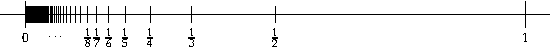
\includegraphics{../figures/oneovernset.pdf}
\end{center}

\medskip
\pause

\textbf{Proof:}
$A \coloneqq \{ \nicefrac{1}{n} : n \in \N \}$ is nonempty.

\medskip
\pause

$\nicefrac{1}{n} > 0$ for all $n \in \N$ \wthus $0$ is a lower bound

\medskip
\pause

\thus \quad
$b \coloneqq \inf\, A$ exists and $b \geq 0$.

\medskip
\pause

Let $a > 0$ be arbitrary.

\medskip
\pause

Archimedean property \wthus $\exists n \in \N$ such that $na > 1$
\pause
\wthus
$a > \nicefrac{1}{n} \in A$

\medskip
\pause

\thus \quad $a$ is not a lower bound \pause \wthus $b=0$.
\qed

\end{frame}

\begin{frame}
For $A \subset \R$, $x \in \R$ define
\quad $x + A  \coloneqq \{ x+y \in \R : y \in A \}$ \quad
$xA  \coloneqq \{ xy \in \R : y \in A \}$.

\medskip
\pause

E.g., if $A = \{ 1,2,3 \}$, then $5+A = \{ 6,7,8 \}$ and $3A = \{ 3,6,9
\}$.

\pause

\begin{proposition}
Let $A \subset \R$ be nonempty.
\begin{enumerate}[(i)]
\item If $x \in \R$ and $A$ is bounded above, then $\sup (x+A) = x + \sup\, A$.
\item \pause If $x \in \R$ and $A$ is bounded below, then $\inf (x+A) = x + \inf\, A$.
\item \pause If $x > 0$ and $A$ is bounded above, then $\sup (xA) = x ( \sup\, A )$.
\item \pause If $x > 0$ and $A$ is bounded below, then $\inf (xA) = x ( \inf\, A )$.
\item \pause If $x < 0$ and $A$ is bounded below, then $\sup (xA) = x ( \inf\, A )$.
\item \pause If $x < 0$ and $A$ is bounded above, then $\inf (xA) = x ( \sup\, A )$.
\end{enumerate}
\end{proposition}

\pause

Note that if $x < 0$, then for multiplication supremum and infimum switch.

\end{frame}

\begin{frame}

\textbf{Proof:}
Let's prove (i):

``If $x \in \R$ and $A$ is bounded above, then $\sup (x+A) = x
+ \sup\, A$'',

rest are exercises.

\medskip
\pause

Suppose $b$ is an upper bound for $A$.

\medskip
\pause

\thus \quad
$y \leq b$ for all $y \in A$
\wthus
$x+y \leq x+b$ for all $y \in A$

\medskip
\pause

\thus \quad $x+b$ is an upper bound for $x+A$.

\medskip
\pause

If $b = \sup\, A$, then
\quad
$\sup (x+A) \leq x+b = x+ \sup\, A$.

\medskip
\pause

Opposite inequality is similar:
\quad
\pause
Suppose $c$ is an upper bound for $x+A$.

\medskip
\pause

\thus \quad $x+y \leq c$ for all $y \in A$
\pause
\wthus
$y \leq c-x$ for all $y \in A$

\medskip
\pause

\thus \quad
$c-x$ is an upper bound for $A$.

\medskip
\pause

If $c = \sup (x+A)$, then \quad
$\sup\, A \leq c-x = \sup (x+A) -x$.
\qed

\end{frame}

\begin{frame}
\begin{proposition}
Let $A, B \subset \R$ be nonempty sets such that $x \leq y$ whenever $x \in A$ and
$y \in B$.
\pause

Then $A$ is bounded above, $B$ is bounded below, and $\sup\, A \leq \inf\, B$.
\end{proposition}

\pause

\textbf{Proof:}
Any $x \in A$ is a lower bound for $B$.

\medskip
\pause

\thus \quad
$x \leq \inf\, B$ for all $x \in A$

\medskip
\pause

\thus \quad
$\inf\, B$ is an upper bound for $A$

\medskip
\pause

\thus \quad
$\sup\, A \leq \inf\, B$.
\qed

\bigskip
\pause

Care must be taken with suprema and infima and strict inequalities.

\medskip
\pause

``$x < y$ for all $x \in A$ and $y \in B$''
still only implies $\sup\, A \leq \inf\, B$ (nonstrict).

\medskip
\pause

E.g., $A \coloneqq \{ 0 \}$ and $B \coloneqq \{ \nicefrac{1}{n} : n \in \N \}$
\pause
\wthus $0 < \nicefrac{1}{n}$ for all $n \in \N$.

\medskip
\pause

However, $\sup\, A = 0$ and $\inf\, B = 0$.
\end{frame}

\begin{frame}


\begin{proposition}
If $S \subset \R$ is nonempty and bounded above,
then for every $\epsilon > 0$ there exists an $x \in S$ such
that $(\sup\, S) - \epsilon < x \leq \sup\, S$.
\end{proposition}

\pause

Proof is an exercise.

\end{frame}

\begin{frame}

%To make using suprema and infima even easier, we may want to
%write $\sup\, A$ and $\inf\, A$ without worrying about $A$ being
%bounded and nonempty.  We make the following natural definitions.

\begin{definition}
Let $A \subset \R$ be a set.
\begin{enumerate}[(i)]
\item \pause If $A$ is empty, then \quad $\sup\, A \coloneqq -\infty$.
\item \pause If $A$ is not bounded above, then \quad $\sup\, A \coloneqq \infty$.
\item \pause If $A$ is empty, then \quad $\inf\, A \coloneqq \infty$.
\item \pause If $A$ is not bounded below, then \quad $\inf\, A \coloneqq -\infty$.
\end{enumerate}
\end{definition}

\pause
\textbf{Remark:}
$\infty$ and $-\infty$ are sometimes treated as numbers.  

\medskip
\pause

$\R^* \coloneqq \R \cup \{ -\infty , \infty\}$ (extended real numbers)
is an ordered set

($-\infty < \infty$ \quad and \quad
$-\infty < x$ and $x < \infty$ for all $x \in \R$).

\medskip
\pause

Some (but not all) arithmetic can be done in the obvious way,

\medskip
\pause

leave
$\infty-\infty$, $0 \cdot (\pm\infty)$, and $\frac{\pm\infty}{\pm\infty}$
undefined.

\medskip
\pause

We avoid using this arithmetic;
$\R^*$ is not a field!

\end{frame}

\begin{frame}
If $A \not= \emptyset$ is finite, then
$\inf A \in A$
and
$\sup A \in A$.

\medskip
\pause

We then usually write

\medskip

$\min\, A \coloneqq \inf\, A$ \qquad (minimum)

\medskip

$\max\, A \coloneqq \sup\, A$ \qquad (maximum)

\medskip
\pause

E.g., \qquad
$\max \{ 1,2.4,\pi,100 \} = 100$ \qquad
$\min \{ 1,2.4,\pi,100 \} = 1$.
\end{frame}

\begin{frame}
Some exercises with useful conclusions.

\medskip
\pause

\textbf{Exercise:}
Prove that
if $t \geq 0$ ($t \in \R$), then there exists an $n \in \N$ such that $n-1 \leq t < n$.

\medskip
\pause

\textbf{Exercise:}
Let $x, y \in \R$.  Suppose $x^2 + y^2 = 0$.  Prove that 
$x = 0$ and $y = 0$.

\medskip
\pause

\textbf{Exercise:}
Let $A$ and $B$ be two nonempty bounded sets of real numbers.  Let
$C \coloneqq \{ a+b : a \in A, b \in B \}$.
Show that $C$ is a bounded set and that
\begin{equation*}
\sup\,C = \sup\,A + \sup\,B 
\qquad \text{and} \qquad
\inf\,C = \inf\,A + \inf\,B .
\end{equation*}

%\medskip
%
%\textbf{Exercise:}
%Let $A$ and $B$ be two nonempty bounded sets of nonnegative real numbers.
%Define the set
%$C \coloneqq \{ ab : a \in A, b \in B \}$.
%Show that $C$ is a bounded set and that
%\begin{equation*}
%\sup\,C = (\sup\,A )( \sup\,B) 
%\qquad \text{and} \qquad
%\inf\,C = (\inf\,A )( \inf\,B).
%\end{equation*}

\medskip
\pause

\textbf{Exercise:}
Prove the so-called \emph{Bernoulli's inequality}: If $1+x > 0$, then
for all $n \in \N$, we have $(1+x)^n \geq 1+nx$.

\end{frame}

\end{document}
